\documentclass[times, utf8, seminar]{fer}
\usepackage{booktabs}
\usepackage{subcaption}
\usepackage[utf8]{inputenc}
\graphicspath{ {./photos/} }

\begin{document}

% TODO: Navedite naslov rada.
\title{Identifying Depression with Machine Learning}

% TODO: Navedite vaše ime i prezime.
\author{Ivan Lovrenčić}

% TODO: Navedite ime i prezime mentora.
\voditelj{Jan Šnajder}

\maketitle

\tableofcontents

\chapter{Introduction}

Mental health has become a burning matter in the last several years. Currently, there are more people than ever being diagnosed with some kind of mental illness. Furthermore, it has been reported that not only there are more diagnosed patients, but there is a distressing amount of people living with an undiagnosed mental disorder.\footnote{https://www.mentalhealth.org.uk/statistics/mental-health-statistics-people-seeking-help}

Official figures report that from 2005 to 2017 the rate of adolescents reporting symptoms of major depressive disorder increased by more than 52\%.\footnote{https://www.sciencedaily.com/releases/2019/03/190315110908.htm} Some papers are even proclaiming an increase of 80\%. It's apparent that there is an upward trend that will probably resume in the following years. 

In response to these facts, there has been an increasing desire to spread awareness about peoples' mental well-being. However, because of the relatively mild or hidden symptoms, there is still a lot of young people who unknowingly suffer from a variety of mental illnesses like depression, anxiety, etc.\footnote{https://www.psychologytoday.com/us/blog/think-act-be/201705/can-you-be-depressed-without-knowing-it-i-was} 

To provide help in this situation, a research team from John Hopkins University published a paper "Identifying depression on Twitter". The paper's primary goal is to aid with the identification of early symptoms of depression. They used machine learning and natural language processing tools to gain useful information from user's tweets. Finally, they ended up with a model that identifies tweets from depressed users with 86 percent accuracy. 

I believe this is indeed a step in the right direction. Because of that, in this paper, we will go over their results and all the crucial tools that were applied. However, it should be noted that their paper did not solve all of the mentioned challenges. There are unreported issues behind that glamourous score, as we will mention in the following chapters. Furthermore, we will recreate their experiments and do the same evaluations. Lastly, we will compare the acquired and original results to make a final conclusion.

\chapter{Relevant work}

The main topic of this paper is the reevaluation of the paper "Identifying Depression on Twitter".  We also will use it as a guideline, as we reimplement their models and compare the final results. To understand those results better, I believe it is important to clarify the researchers' motivation for investigating that topic in the first place.

At the beginning of their paper, the researchers explain that depression is currently, the world's most prevalent mental illness and that it has affected more than 80 million Americans in 2015 alone \citep{depression}. They continue by pointing out that the way the depression is diagnosied has not significantly changed in over half of a century. With that as their motivation, they worked on a strategy to simplify that diagnostic process. 

For starters, they aimed to create a model that would accurately classify tweets into two classes - tweets written by depressed and non-depressed users. To achieve that goal, they used a variety of shallow machine learning algorithms like decision trees, support vector machines (SVM), logistic regression, etc \citep{depression}. Naturally, to obtain useful information from the text, they had to use natural language processing (NLP) tools. 

The main and only NLP tool the authors used was the bag-of-words method. In their case, it was sufficient, as they had notably high accuracy and precision. Nevertheless, I think they should have tried a few additional tools to get a feeling of what approach could potentially have a more prominent impact. 

In the end, researchers concluded that this is a new domain and there is a lot of area for improvement. They believe that this research could eventually provide more insight into how mental disorders are related to one's textual expression. 

\chapter{Machine Learning}

Machine learning (ML) and NLP are the two fundamental elements of Johns Hopkin's paper "Identifying Depression of Twitter". In practice, researchers often use NLP alongside machine learning, as it is shown by numerous state-of-the-art models. Furthermore, in recent years, machine learning's subclass, deep learning, has become remarkably successful.\footnote{https://medium.com/@andersasac/dominance-of-deep-learning-39e5cc571ab5} However, Johns Hopkins's paper is entirely focused on shallow ML algorithms like SVMs, logistic regression, decision trees, etc. Consequently, that will also be the topic of this chapter, where we will explain, in more detail, some of the mentioned algorithms.

Most of the ML algorithms rely on building a precise mathematical model that is based on some sample data.\footnote{https://en.wikipedia.org/wiki/Machine\_learning} There are a few ways we can group those algorithms, but the most common one is by algorithms "learning" technique. Therefore, we divide them into - supervised and unsupervised algorithms.

On the one hand, supervised algorithms are applied when we are presented with data that has both the example $x$ and the corresponding label $y$. That is commonly written like a mapping function \textit{y = f(x)}.\footnote{https://en.wikipedia.org/wiki/Supervised\_learning} On the other hand, when we are dealing with unstructured data that is not labeled, we use unsupervised learning. In those situations, we ordinarily have only the examples, without the analogous labels.\footnote{https://en.wikipedia.org/wiki/Unsupervised\_learning} In the case of Johns Hopkins's paper, they have only applied the supervised approach hence why we are going to focus only on that field from now.

\newpage

Amongst supervised ML algorithms, we can point out one more notable difference. Namely, I am referring to the division between classification and regression algorithms. As they both belong to the supervised ML tools, they both share the same concept of utilizing the known dataset. Specifically, they both use the examples and matching labels. The only difference is that in classification labels are discrete, whereas, in regression, they are continuous values.  


Figure 3.1 accurately illustrates a visual difference between classification and regression approaches. A convenient way of perceiving that difference would be in the context of the weather prediction model. In that case, a regression model would predict the exact value of a temperature, whereas the classification model would predict a discrete value, like cold or hot weather.

\begin{figure}[h]
	\centering
	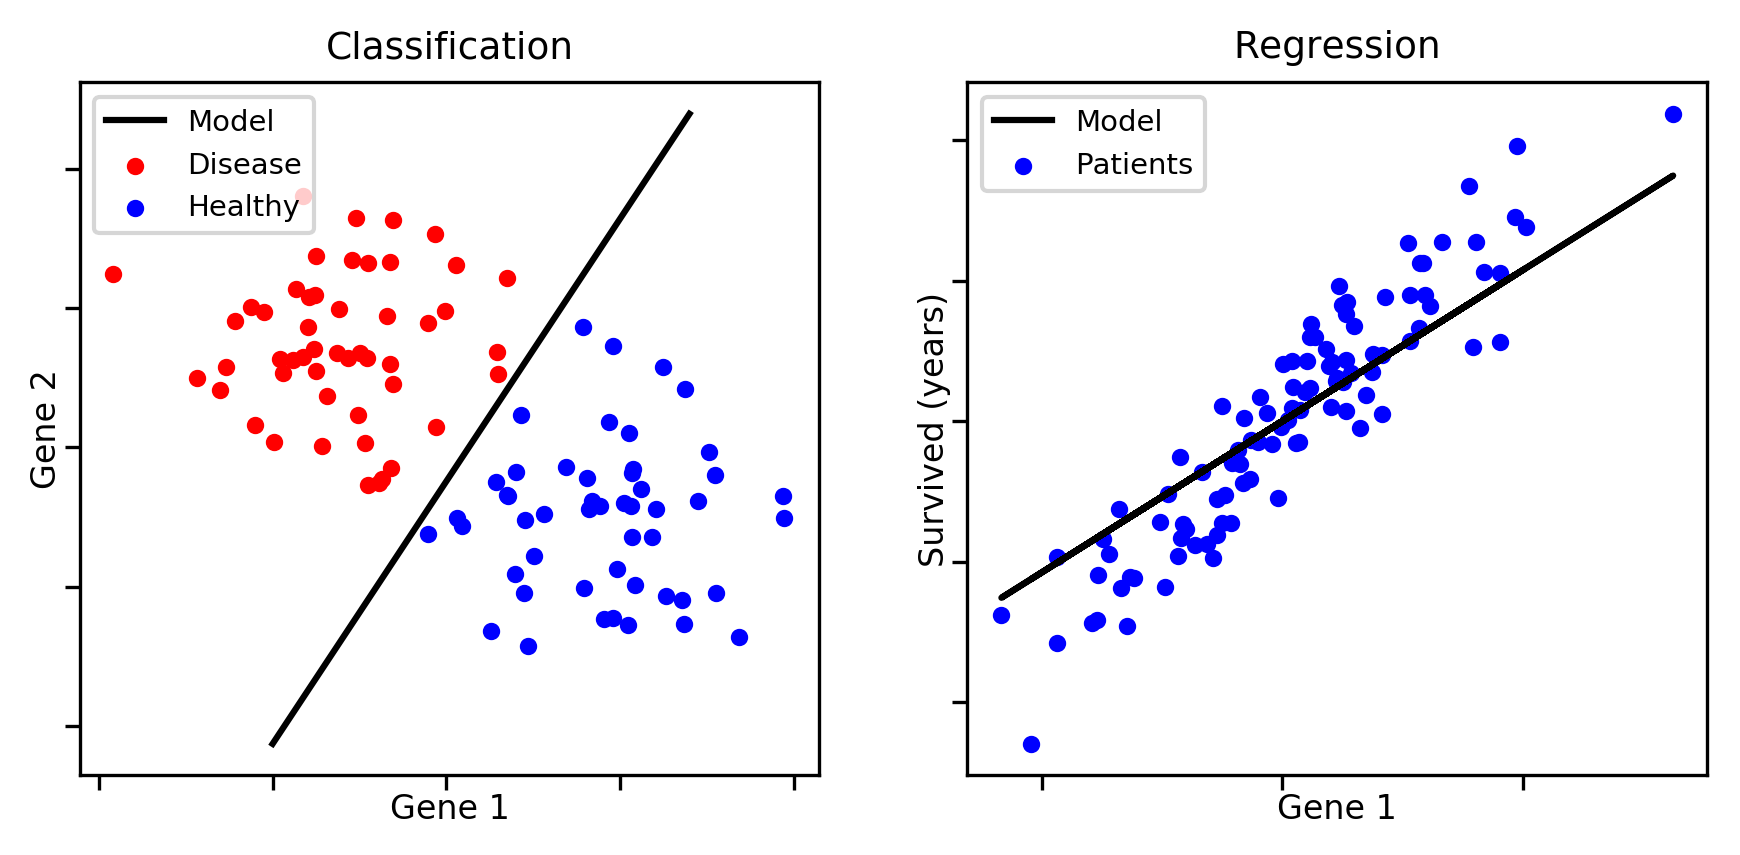
\includegraphics[width=14cm]{classification}
	\caption{An example of classification and regression. Here we are modeling people's well-being in regards to the presence of certain genes. \protect \footnotemark}
\end{figure}

\footnotetext{https://dev.to/petercour/machine-learning-classification-vs-regression-1gn}

In the case of Johns Hopkins's paper, we have a typical example of a supervised classification problem. Specifically, they have built a model that classifies tweets in one of two discrete classes. As mentioned, those classes are - depressed and non-depressed users. To accomplish that, they had to use a few of the available classification algorithms. We'll start with the first one - decision tree.

\newpage

\section{Decision tree}

Decision trees are one of the simpler and broadly used classification algorithms. They are recognizable by their clarity and interpretable nature. Moreover, they do not demand a lot of data preparation, and they are not computationally costly. 

The decision tree's original premise is remarkably simplistic. We want to detect the nodes (node represents a feature) that provide the most information about the dataset and to position those nodes higher on the tree hierarchy. In other words, the aim is to find features that differentiate between classes the most. Although there can be a difference in the way the final solution is determined, most of the decision trees' algorithms work similarly.

\begin{figure}[h]
	\centering
	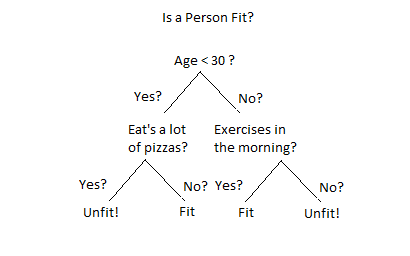
\includegraphics[width=9cm]{decision-tree}
	\caption{An example of simple decision tree that is modeling whether the person is fit or not.  \protect \footnotemark}
\end{figure}

\footnotetext{https://medium.com/greyatom/decision-trees-a-simple-way-to-visualize-a-decision-dc506a403aeb}

Figure 3.2 displays a simple decision tree. There we can notice that the most influential node in that tree is age node. We can conclude that from the fact that based on the decision of that node, we are effectively dismissing nearly half of the decision tree. In other words, the highest node has the most substantial decision. As we move down the tree, the nodes are becoming less and less significant. In the end, we are left with the leaves (last nodes of the tree), where we will find labels for our examples. As mentioned, there are a few algorithms that can be used to calculate this solution, and most of them rely on entropy and information gain estimation.

In conclusion, we can notice that the decision trees bring a few notable advantages. Mainly, their simplicity and interpretable structure. However, those benefits come with a cost. Decision trees are not used in any state-of-the-art models, as they usually have poor performance on more complicated tasks that require a lot of features.

\newpage

\section{Logistic regression}

Logistic regression, although the name implies otherwise, is an effective classification model. Specifically, logistic regression belongs to the family of generalized linear models (GLM). GLMs represent a variety of ML models that share a few distinct characteristics.  Firstly, the most notable trait they share is linearity. Specifically, this means that their division line will be linear in the examples vector space. Secondly, although they are linear models, they do not have a linear activation function. In the case of logistic regression, we use the sigmoid function \citep{logistic}.

\begin{figure}[h]
	\centering
	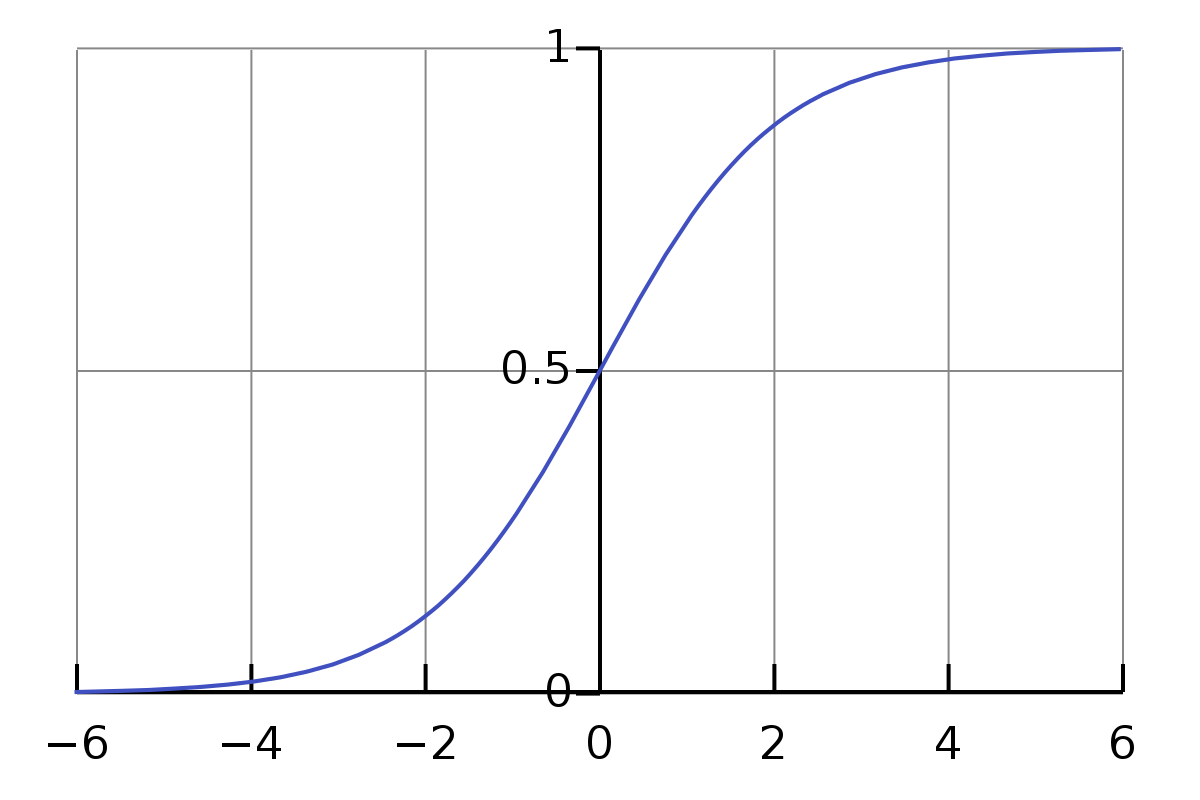
\includegraphics[width=8cm]{sigmoid}
	\caption{Sigmoid function \protect \footnotemark}
\end{figure}

\footnotetext{https://en.wikipedia.org/wiki/Sigmoid\_function}

Now, it is necessary to remark, why do we need a non-linear activation function? To answer that, we have to take a look at linear regression. Linear regression is a simpler model used for classification and regression tasks. However, in the case of classification, linear regression displays a specific challenge. 

\begin{equation}
	h(x; w) = w^{T}x 
\end{equation}

To better understand, let's have a closer look at the linear regression model. Equation 3.1 shows us the details. As we can notice, we have a vector $w$, that represents weights, and an example $x$. The way we do classification is as follows: we calculate the dot product of the example $x$ and transposed weights vector $w$, then we compare acquired results with some fixed value (usually, that value is zero). Finally, we classify an example based on that comparison. So, what is the challenge I mentioned?

\newpage

\begin{equation}
L(y^{(i)}, h(\textbf{x}^{(i)})) = (y^{(i)} - h(\textbf{x}^{(i)}))^2
\end{equation}

Figure 3.4 clearly illustrates the problem. Namely, linear regression has a problem with outliers. As we can see from the figure, if we introduce values that are not close to the class divider line, linear regression performs inadequately. Why is that? Specifically, the linear regression loss function is a quadratic function (equation 3.2), which means that if we have an example $x$ that is an outlier, we get a high loss ($h(x)$ grows bigger as an example is further from the divider line). In other words, even though we classify examples correctly, the difference between the label $y$ (usually some discrete value like 0 or 1) and the model's output $h(x)$ will be enormous for the examples that are far from the divider line. To optimize that loss, the model has to readjust, and in the process of doing that, ends up classifying poorly.    \footnote{https://jinglescode.github.io/datascience/2019/05/07/why-linear-regression-is-not-suitable-for-classification/}

\begin{figure}[h]
	\centering
	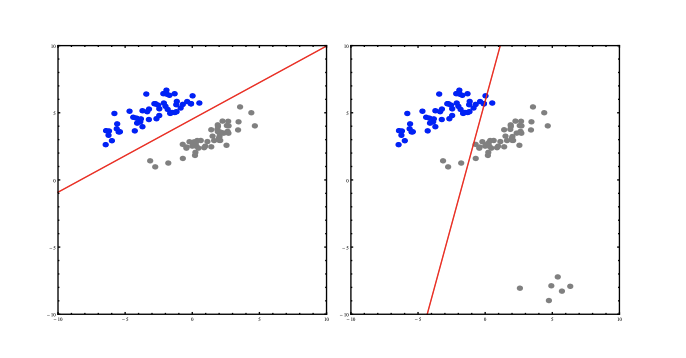
\includegraphics[width=12cm]{linear-regression}
	\caption{Example of linear regression reaction to outliers \protect \footnotemark}
\end{figure}

\footnotetext{https://www.fer.unizg.hr/predmet/su/materijali\#\%23!p\_rep\_34381!\_-159820}

How will the sigmoid function solve this? 
For starters, let's have a look at figure 3.3. As we can notice, the sigmoid function has a range between one and zero. So, if we would map the model's output into the sigmoid function, our output would also be in the range between one and zero. This feature would prevent those huge losses from outliers we had earlier. Moreover, the sigmoid function gives us a probabilistic output. We want that because probabilistic output offers a precise way of knowing to which class the example belongs. 

\begin{equation}
	L(y,h(\textbf{x})) = - y*ln((\textbf{x})) - (1-y)*ln(1-h(\textbf{x}))
\end{equation}

All those mentioned advantages lead to one conclusion - logistic regression is a robust and powerful model. Figure 3.5 perfectly visualizes that claim. There we can notice that logistic regression (the red line) is more sturdy and still performs flawlessly in the presence of outliers. That performance is also backed up by its cross-entropy loss function, where we can see that now, we do not have huge losses for correctly classified outlier values (equation 3.3). 


\begin{figure}[h]
	\centering
	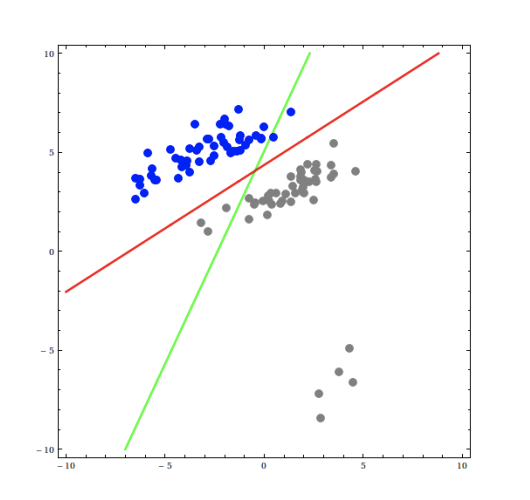
\includegraphics[width=8cm]{logistic}
	\caption{Difference between logistic regression(red line) and linear regression(green line) \protect \footnotemark}
\end{figure}

\footnotetext{https://www.fer.unizg.hr/predmet/su/materijali\#\%23!p\_rep\_34381!\_-159820}

All in all, we can see that logistic regression is a reliable classification tool. It's robust to outliers and, because we use a sigmoid as activation function, we have the probabilistic output from the model. On the other hand, linear regression should not be used for classification, as it carries certain difficulties with its approach.

\newpage

\section{Support vector machine}

Support vector machines (SVMs) are one of the most powerful tools in the machine learning toolbox. The idea behind SVMs originates from the desire for more reliable generalization in classification. The model has better generalization power when it's performing suitably on unseen datasets. To improve that ability, researchers introduced a concept - the model will generalize better if the division line between classes is maximumly separated. In other words, we want our model to split the data with a hyperplane that is the furthest from all classes \citep{svm}. 

\begin{figure}[h]
	\centering
	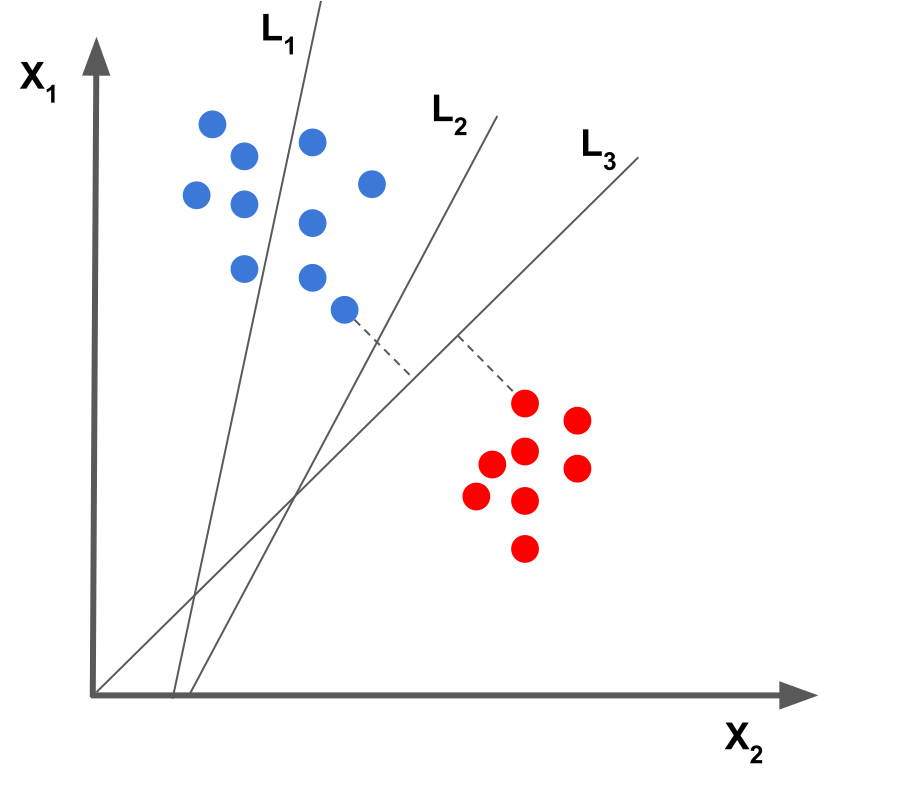
\includegraphics[width=9cm]{svm}
	\caption{Both lines L2 and L3 are perfectly seperating two classes, but only the line L3 is maximumly distant from both classes. \protect \footnotemark}
\end{figure}

\footnotetext{https://www.learnopencv.com/support-vector-machines-svm/}


The idea we just expressed is often defined as a maximum margin hyperplane problem. Figure 3.6 excellently describes that approach. There we can notice that although there are a couple of models (the divider line is just a model) that are separating the dataset, only the L3 model has the maximum margin hyperplane. Moreover, figure 3.7 displays a comparison between logistic regression and SVM. As we can notice, both logistic and SVM are classifying all the examples correctly. However, only SVM insists on the maximum margin, while logistic regression doesn't.

\begin{figure}[ht]
	\begin{subfigure}{.5\textwidth}
		\centering
		% include first image
		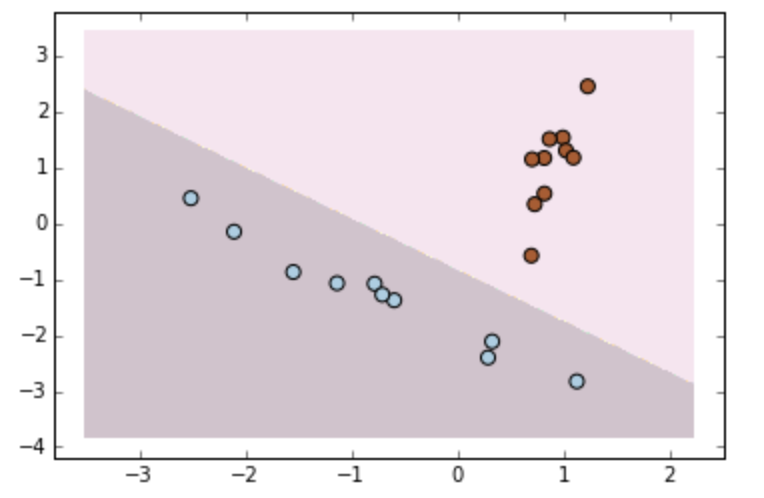
\includegraphics[width=.8\linewidth]{svm-logistic1}  
		\caption{SVM}
		\label{fig:sub-first}
	\end{subfigure}
	\begin{subfigure}{.5\textwidth}
		\centering
		% include second image
		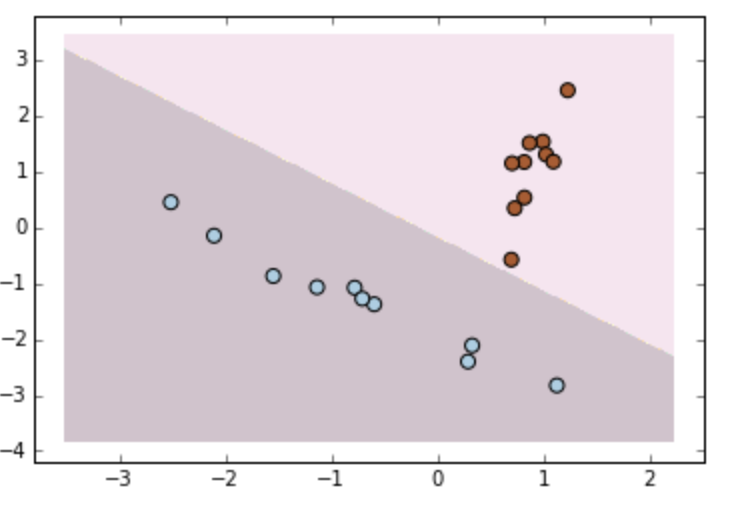
\includegraphics[width=.8\linewidth]{svm-logistic2}  
		\caption{Logistic regression}
		\label{fig:sub-second}
	\end{subfigure}
	\caption{Difference between SVM and logistic regression \protect \footnotemark}
	\label{fig:fig}
\end{figure}


\footnotetext{https://github.com/jsnajder/MachineLearningTutorial/blob/master/Machine\%20Learning\%20Tutorial.ipynb}

In its primary form, SVM is a linear model. However, the data we are trying to classify will not always be linearly separable. Namely, it is impossible to split a dataset with the maximum margin hyperplane, if the dataset is not linearly separable. In other words, we can not divide the dataset, if we can't draw a straight line through it, that will separate it in the individual classes \citep{svm}.

\begin{figure}[h]
	\centering
	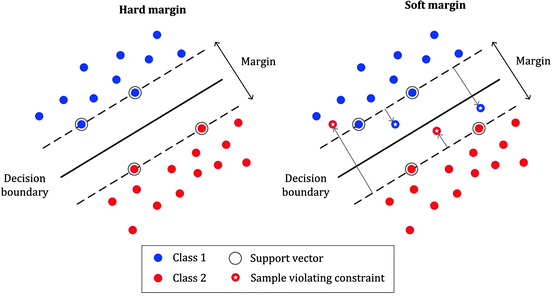
\includegraphics[width=12cm]{margin}
	\caption{Difference between hard-margin (left) and soft-margin (right) model. \protect \footnotemark}
\end{figure}

\footnotetext{https://mc.ai/math-behind-svmsupport-vector-machine/}

To solve that problem, researchers had to introduce two variants of the maximum margin model. The initial version, which we described at the beginning, is the hard-margin model. In that variant, the data has to be linearly separable, otherwise, the model will not be able to find any solution. On the other hand, we have the soft-margin model. The soft-margin model is a balance between maximum margin and finding the optimal solution in a linearly non-separable dataset.

Figure 3.8 nicely illustrates the difference between them. On the left side, we have a hard-margin model, and, as we can notice, it does not allow examples inside the margin space. Furthermore, we can also notice that hard-margin always has to be a hundred percent accurate. If there isn't a hyperplane that can achieve that, the SVM will not find the solution. On the other hand, the soft-margin model permits examples inside the margin and, more importantly, it also allows incorrect classifications. Because of that, soft-margin is the default version of the algorithm we get when we use SVMs from most of the accessible ML libraries \citep{fradkin2006}.

\begin{figure}[h]
	\centering
	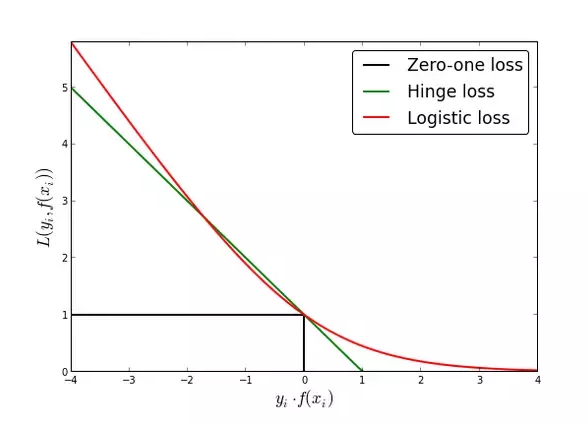
\includegraphics[width=12cm]{hinge-loss}
	\caption{Hinge loss vs logistic loss function \protect \footnotemark}
\end{figure}

\footnotetext{https://towardsdatascience.com/a-guide-to-neural-network-loss-functions-with-applications-in-keras-3a3baa9f71c5}

Lastly, we are going to mention the SVM loss function (equation 3.4). The SVM loss function is generally known as a hinge loss. In the previous chapters, we have mentioned quadratic loss (linear regression) and cross-entropy loss (logistic regression).  In comparison to quadratic loss, hinge loss is also an improvement, as it strikes one of more reliable loss functions.

\begin{equation}
L(y,h(\textbf{x})) = max(0, 1 - y*h(\textbf{x}))
\end{equation}

Figure 3.9 illustrates a comparison between zero-one, hinge, and logistic loss.  Zero-one represents a perfect loss function that would only "punish" the model for the incorrectly classified examples. However, that loss function is not derivable, so it is not suitable for usage. The next best thing would be the hinge or logistic loss. They both have their advantages and flaws, yet there is not a clear winner. Hinge loss theoretically offers greater precision, since it "punishes" way more the incorrectly classified than the correctly classified examples. However, logistic loss offers the probabilistic output, which could be useful in various ML tasks. 

To conclude, we can see that SVMs are an effective tool in ML toolbox. They are robust and, more importantly, they have outstanding generalization power. However, they do have some shortcomings. Specifically, they do not respond well to class imbalance, so it is advised to check for the alternative in those kinds of scenarios.

\newpage

\section{Naïve Bayes}

Naive Bayes is our first generative ML model. That means we are making another major differentiation amongst ML algorithms. In this case, we are separating them between discriminative and generative algorithms. So, what is the difference? 

In the last few chapters, we have discussed several ML algorithms. All those algorithms (except decision tree) can be categorized as the discriminative ML algorithms. The most intuitively noticed difference is whether the model is probabilistic. But, there are going to be some exceptions. For example, support vector machines, as mentioned, do not have a probabilistic output. On the other hand, logistic regression has. However, it is not entirely identical, like the one from the generative models, as we will explain it in the following part.

\begin{equation}
P(\textbf{x},y) = p(\textbf{x}|y)*P(y) 
\end{equation} \newline

In classification algorithms, as stated, we have examples and corresponding labels. Most discriminative algorithms, if they are probabilistic, represent the probability as \textit{a posteriori} probability. On the other hand, generative models ordinarily follow their generative story. In short, that is the story about how did the data come to be. That story, in the case of Naive Bayes, is modeled by the joint probability distribution (equation 3.5). However, although they are not modeling the \textit{a posteriori} probability directly, most of the generative models, including the Naive Bayes, classify by calculating the \textit{a posteriori} from the joint probability distribution. In the case of Naive Bayes, we do it by using the Bayes' theorem.


\begin{equation}
P(y|x) = \frac{p(x|y)*P(y)}{P(x)}
\end{equation} \newline


The Bayes' theorem is one of the most famous theorems in ML.  Equation 3.6 shows us the details. Specifically, we can define the next probabilities: 

\begin{itemize}
	\item $P(y|x)$ - the probability of label $y$ for an example x (a posteriori)
    \item $P(y)$ - the probability of label $y$ (a priori)
    \item $P(x)$ - the probability distribution of the examples (sometimes not included when we are just classifying )
	\item $P(x|y)$ - the probability of example $x$ if there is a label $y$ (likelihood)
\end{itemize}

As we can see, this can be directly applied to the dataset. Furthermore, we can even formalize this more elegantly, and write it to describe the Naive Bayes model.

\begin{equation}
h(\textbf{x;}\theta) = P(y = j | \textbf{x}) = \frac{ p(\textbf{x}| y = j) P(y = j)}{ \sum_{k} p(\textbf{x} | y = k ) P(y = k)}
\end{equation} \newline

As we can notice from equation 3.7, Naive Bayes will, for a given example $x$, calculate the probability of that example being labeled with a label $j$. To estimate that probability, we have to determine what are the specific probabilities that comprise the Bayes theorem.

\begin{figure}[h]
	\centering
	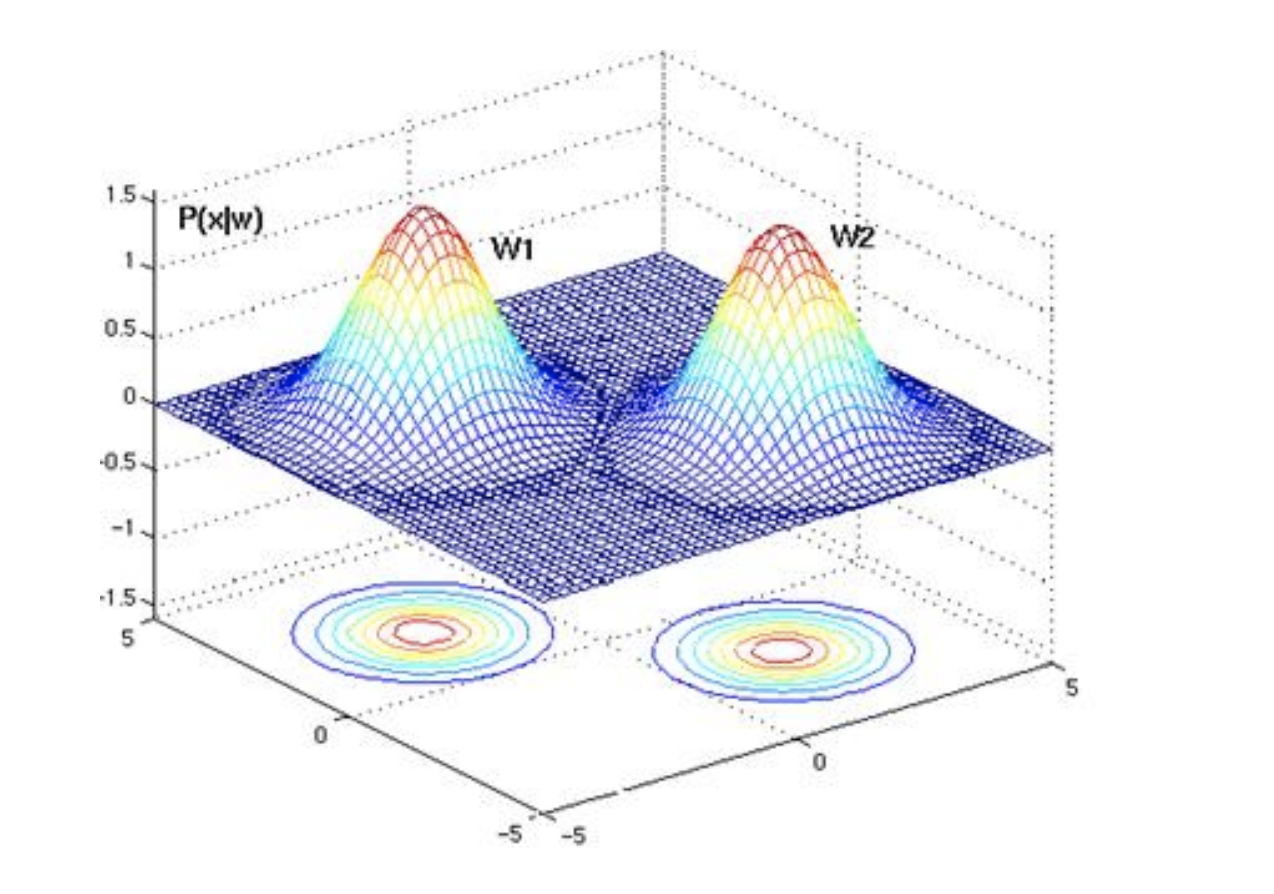
\includegraphics[width=12cm]{bayes}
	\caption{Binary classification with normal distributions for class likelihood P(x|y) \protect \footnotemark}
\end{figure}

\footnotetext{https://www.fer.unizg.hr/\_download/repository/SU-2019-15-BayesovKlasifikator.pdf}


To determine those probabilities, we will have to use parameter estimation. Parameter estimation is a group statistical method with which we are estimating the parameters of the probability distributions. Often, those distributions, largely depend on the data. So, for example, for continuous data like temperature or student's height, we would model it with the normal distribution. Then, we would use one of the methods from parameter estimation, like the maximum likelihood estimation (MLE), and we would estimate the parameters of that normal distribution. In the process of estimating those parameters, we are effectively training the model. 

\chapter{Data and model}

\section{Dataset}

In this chapter, we are going over the dataset that was used in Johns Hopkins paper "Identifying Depression on Twitter". For starters, the dataset was collected from the Shared task organizers of the CLPsych 2015. The dataset itself comprises of the 1000 twitter users, for which there are up to 3000 individual tweets \citep{clpsych}.  Amongst those 1000 users, 574 users have no mental health condition, and 326 users have a major depressive disorder (MDD). For their research, that resulted in 1,253,594 tweets as a control variable (from users who are not depressed), and 742,560 tweets with a depression. 

\begin{table}[h!]
	\centering
	\begin{tabular}{|p{3cm}|p{3cm}|p{3cm}|} 
		\hline
		\multicolumn{3}{|c|}{CLPsych 2015 Twitter dataset}\\
		\hline
		Mental condition & Number of users & Number of tweets \\ [0.5ex] 
		\hline
		No condition & 574 & 1,253,594 \\ 
		Depression & 326 & 742,560 \\
		\hline
		\textbf{Total} & \textbf{1000} & \textbf{2,000,000}\\
		\hline
	\end{tabular}
	\caption{Distribution of the CLPsych 2015 dataset}
	\label{Table:1}
\end{table}

For this paper, I could not obtain the originally used CLPscych dataset. There were a few GDPR and sensitive data concerns that could not be solved in such a short amount of time I had to write this paper. However, I did find a dataset that could work as a replacement. The dataset I found is the Reddit Self-Reported Depression Diagnosis (RSDD) dataset, from Georgetown University. The RSDD dataset consists of 126,000 users, amongst which 9000 users are the depressed users, and 107,000 users are the control users \citep{rsdd}. However, for this paper, I have only used a portion of that dataset. Specifically, I have only used 892 users from the dataset, as I found it acceptable for this paper. Furthermore, I have divided the dataset into train, validation, and test sets. Tables 4.2 and 4.3 display the dataset division.


\newpage

\begin{table}[h!]
	\centering
	\begin{tabular}{|p{3cm}|p{3cm}|p{3cm}|} 
		\hline
		\multicolumn{3}{|c|}{Reddit Self-Reported Depression Diagnosis (RSDD) dataset}\\
		\hline
		Data split & Number of users & Number of posts \\ [0.5ex] 
		\hline
		Train & 486 & 295,509 \\ 
		Validation  & 206 & 118,937 \\ 
		Test & 200 & 117,899  \\
		\hline
		\textbf{Total} & \textbf{892} & \textbf{532,345}\\
		\hline
	\end{tabular}
	\caption{Distribution of the RSDD dataset based on data split}
	\label{Table:1}
\end{table}

As we can notice from table 4.3, the RSDD has a more prominent class imbalance than the CLPsych dataset. However, the biggest contrast is in the style of the document. On the one hand, we have tweets, which are limited to 140 characters. On the other hand, we have Reddit posts, which can be, on average, three times longer.\footnote{https://expandedramblings.com/index.php/reddit-stats/} That disbalance solely requires different methods of text preprocessing and feature extraction. However, in this paper, we will do the same reevaluations as them, only with this new dataset. That way, we will examine whether the Johns Hopkins approach can be applied to the different textual formats and the new domains. \newline

\begin{table}[h!]
	\centering
	\begin{tabular}{|p{3cm}|p{3cm}|p{3cm}|} 
		\hline
		\multicolumn{3}{|c|}{Reddit Self-Reported Depression Diagnosis (RSDD) dataset}\\
		\hline
		Mental condition & Number of users & Number of posts \\ [0.5ex] 
		\hline
		No condition & 755 & 450864 \\ 
		Depression  & 137 & 81761 \\ 
		\hline
		\textbf{Total} & \textbf{892} & \textbf{532,345}\\
		\hline
	\end{tabular}
	\caption{Distribution of the RSDD dataset based on mental condition}
	\label{Table:1}
\end{table}

\section{Model}

For this paper, I have decided to reimplement all models from Johns Hopkins paper. They have developed several binary classifiers, that were dependent on the shallow ML algorithms, we have mentioned earlier. In total, they have developed five different models. For each model, they combined one of the shallow ML algorithms with the NLP feature extraction tool. In their case, the only tool that was used is the bag-of-words method. For the implementation of those models, I have used the sckit-learn libraries \citep{python}. The entire reimplementation was written in Python 3. 

\subsection{Features}

To utilize the power and effectiveness of the mentioned ML models, firstly, we need to implement the preprocessing and the feature extraction tools. As mentioned, in the case of Johns Hopkins paper, they have only used the bag-of-words (BoW) method. The BoW method is simplistic and extremely easy to implement. The concept of the BoW is as follows: we first collect all the available textual data. Then, we build a vocabulary of that data, and then we map the number of word appearances to those specific words inside the text.\footnote{https://towardsdatascience.com/a-simple-explanation-of-the-bag-of-words-model-b88fc4f4971} Finally, we are left with a vector whose numbers represent a number of occurrences of that specific word. Figure 4.1 nicely illustrates the concept. \newline


\begin{figure}[h]
	\centering
	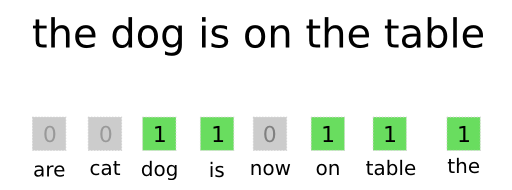
\includegraphics[width=12cm]{bag-of-words}
	\caption{Bag-of-words text representation\protect \footnotemark}
\end{figure}

\footnotetext{https://medium.com/free-code-camp/text-classification-and-prediction-using-bag-of-words-8aeb1396cded}



\chapter{Results}

 The goal of this paper is to successfully reimplement the Johns Hopkins paper "Identifying Depression on Twitter". To accomplish that, firstly, we have to use the same evaluation metrics. Secondly, evaluation results have to be as similar as they can get. In my case, the datasets are not matching. So, by default, my evaluation results should not match the ones from the paper.  However, there should be some similarities. For example, although the results will not be equivalent, I think the rankings among models should stay the same. 

\section{Evaluation}

It is important to evaluate the model in order to check its performance. Depending on the purpose of the model, we can apply different metrics to evaluate it. In the case of Johns Hopkins paper, we have binary classifiers that predict whether the user is depressed or not. In that situation, we would require our models to be as accurate as they can be. However, accuracy is not always the fitting metric. Sometimes, it could be more valuable that our model is more precise, rather than more accurate. 

\begin{figure}[h]
	\centering
	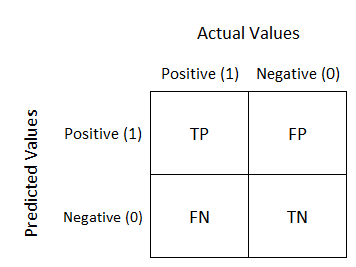
\includegraphics[width=9cm]{confusion-matrix}
	\caption{Confusion matrix \protect \footnotemark}
\end{figure}

\footnotetext{https://towardsdatascience.com/understanding-confusion-matrix-a9ad42dcfd62}

To introduce a more formal description of evaluation metrics, we have to get familiar with a concept of the confusion matrix. The confusion matrix is a specific table layout that allows visualization of the performance of a ML algorithm. Each row of the matrix represents the instances in a predicted class while each column represents the instances in an actual class. Figure 5.1 displays the details.

\newpage

\begin{itemize}
\item \textbf{TP} - true positive = classifier has correctly predicted that this is a positive
\item \textbf{TN} - true negative = classifier has correctly predicted that this is a negative
\item \textbf{FP} - false positive = classifier predicted that this is a positive, whereas it is a negative
\item \textbf{FN} - false negative = classifier predicted that this is a negative, whereas it is a positive 
\end{itemize}


\subsection{Accuracy}

Accuracy is a measure of how much of the predicted labels are correct. In other words, accuracy is the number of correctly predicted examples over the number of all examples. Equation 3.4 shows us a more formal description.

\begin{equation}
Acc = \frac{TP + TN}{TP+TN+FP+FN}
\end{equation} 

\subsection{Precision}

Precision, also called positive predictive value, is the fraction of relevant instances among the retrieved instances. In other words, it is a fraction of positively guessed examples and the sum of all the examples that the model predicted with that label.

\begin{equation}
P = \frac{TP }{TP+FP}
\end{equation} 

\subsection{Recall}

Recall, also known as sensitivity, is the fraction of the total amount of relevant instances that were retrieved. In other words, recall is a fraction of positively predicted examples and the sum of all positively labeled examples.

\begin{equation}
R = \frac{TP }{TP+FN}
\end{equation} 

\subsection{F1-Score}

The F1 score is the harmonic mean of the precision and recall, where an F1 score reaches its best value at 1 (perfect precision and recall). It considers both the precision P and the recall R of the test to compute the score.

\begin{equation}
F1 = \frac{2PR }{P+R}
\end{equation} 

\section{Final results}

In this section, we are going to compare the final results. Table 5.1 displays the results from the Johns Hopkins paper and table 5.2 shows the reimplementation results. 

\begin{table}[h!]
	\centering
	\begin{tabular}{|p{4cm}|p{2cm}|p{2cm}|p{2cm}|p{2cm}|} 
		\hline
		\multicolumn{5}{|c|}{Johns Hopkins paper results}\\
		\hline
		Algorithm & Precision & Recall & F1-score & Accuracy \\ [0.5ex] 
		\hline
		Decision Trees & 0.67 & 0.68 & 0.75 & 0.67 \\ 
		LinearSVC & 0.83 & \textbf{0.83} & 0.83 & 0.82 \\ 
		Naive Bayes & 0.81 & 0.82 & 0.81 & \textbf{0.86} \\ 
		Logistic Regression &  \textbf{0.86} & 0.82 &  \textbf{0.84} & 0.82 \\ 
		Ridge Classifier & 0.81 & 0.79 & 0.78 & 0.79 \\ 
		\hline
	\end{tabular}
	\caption{The evaluation of the Johns Hopkins models}
	\label{Table:1}
\end{table}

\newpage

\begin{table}[h!]
	\centering
	\begin{tabular}{|p{4cm}|p{2cm}|p{2cm}|p{2cm}|p{2cm}|} 
		\hline
		\multicolumn{5}{|c|}{The reimplementation results}\\
		\hline
		Algorithm & Precision & Recall & F1-score & Accuracy \\ [0.5ex] 
		\hline
		Decision Trees & 0.62 & 0.62 & 0.62 & 0.62 \\ 
		LinearSVC & 0.60 & 0.59 & 0.58 & 0.59 \\ 
		Naive Bayes & 0.69 & 0.68 & 0.68 & 0.68 \\ 
		\textbf{Logistic Regression} &  \textbf{0.71} & \textbf{0.70} &  \textbf{0.70} & \textbf{0.70} \\ 
		Ridge Classifier & 0.67 & 0.67 & 0.67 & 0.67 \\ 
		\hline
	\end{tabular}
	\caption{The evaluation of the reimplemented models}
	\label{Table:1}
\end{table}

As predicted, the results are not similar. Reimplementation results are visibly worse by all metrics. Those poor results could be attributed to the document style change. As mentioned, the RSDD dataset uses Reddit post, whereas the Johns Hopkins dataset uses Twitter. As we stated, we have not changed the preprocessing and the feature extraction tools, which could explain the results. 


Furthermore, the prediction that the model rankings would stay the same is partially satisfied. We can see that the best overall model is still logistic regression. Also, most of the other models kept their rankings even on this new dataset. However, there is one surprise. SVM has performed the worst on the new dataset, whereas, on the Johns Hopkins dataset, it was one of the better models. Why is that? 

Well, as discussed, the RSDD dataset has a huge class disbalance, as there is a lot more of non-depressed than depressed users. Because of that disbalance SVM can not determine the optimal solution. As we mentioned in the ML chapter, if there is a case of an imbalanced dataset, it is wise to find a better alternative to SVM.

In conclusion, we can see that the approach from Johns Hopkins paper to a certain degree applies to different datasets and domains. Although we didn't get the state-of-the-art results or even an increase, they were satisfying and in line with the predictions. However, there is clearly a room for an improvement, as there are a lot more features that could be extracted and utilized in this kind of task. 

\chapter{Conclusion}

To help with a burning issue of alarming rates of mental health disorders, the researchers from Johns Hopkins University published a paper "Identifying Depression on Twitter". To add my contribution, I  reimplemented and reviewed their paper. The plan was to successfully reevaluate and to verify that their methods still are suitable and relevant.

Unfortunately, I could not acquire the original dataset, so the one-to-one reevaluation was not possible, as I could not get the equivalent results with a different dataset. Moreover, the datasets do not have the same document style, which consequently brings even more disbalance between the datasets. That disbalance caused most of the models to perform substantially worse. Furthermore, there is also a noteworthy imbalance between classes in the new dataset, which prompted the SVM to perform horribly.

Nevertheless, the results did prove that their approach alone could acquire pleasing results, even in different domains. In the case of this paper, we have demonstrated that although we have used entirely different document styles, the overall results were still pleasing and, most of the results were in line with our predictions.



\bibliography{literatura}
\bibliographystyle{fer}

\end{document}
